% Chapter: 05_fuzzy_interp
% Included from lectures/main.tex

\section{Fuzzy Interpretability}

\begin{frame}{Activation Oracles}
\fullfig{figures/karvonen2026/training.png}{karvonen2026}
\end{frame}

\begin{frame}{Activation Oracles: Benchmarks}
\fullfig{figures/karvonen2026/benchmarks.png}{karvonen2026}
\end{frame}

\begin{frame}{Natural Language Autoencoders}
\fullfig{figures/fraser-taliente2026/training.png}{fraser-taliente2026}
\end{frame}

\begin{frame}{NLAs Reveal Unverbalized Reasoning}
\fullfig{figures/fraser-taliente2026/reward-reasoning.png}{fraser-taliente2026}
\end{frame}

\begin{frame}{NLAs Hallucinate}
\fullfig{figures/fraser-taliente2026/hallucinations.png}{fraser-taliente2026}
\end{frame}

\begin{frame}{NLAs Detect Unverbalized Evaluation Awareness}
\fullfig{figures/fraser-taliente2026/eval-awareness.png}{fraser-taliente2026}
\end{frame}

\begin{frame}{NLAs Win the Auditing Game}
\fullfig{figures/fraser-taliente2026/audit-game.png}{fraser-taliente2026}
\end{frame}

\begin{frame}{Application: Opus 4.8 System Card}
\begin{center}
\Large
In 5\% of sampled RL episodes, Claude Opus 4.8 is internally aware of a grader, but never verbalizes it.
\end{center}
\source{anthropic2026a}
\end{frame}

\begin{frame}{Exercise: Play with an NLA}
\begin{center}
\Large
\href{https://www.neuronpedia.org/llama3.3-70b-it/nla}{neuronpedia.org/llama3.3-70b-it/nla}
\end{center}
\end{frame}

\begin{frame}{The Jacobian Lens}
\centerline{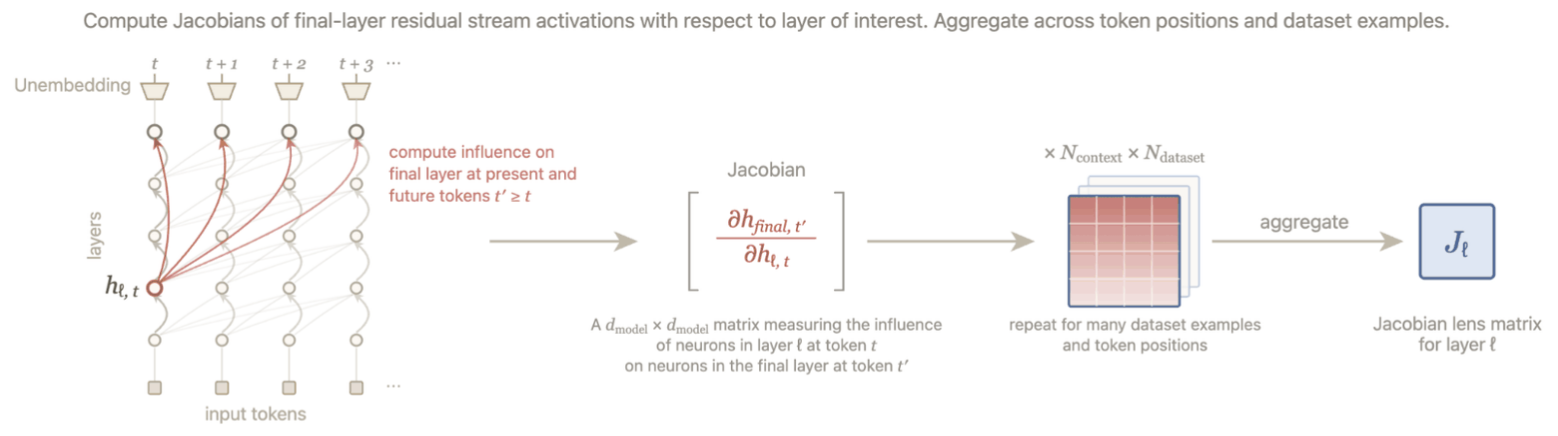
\includegraphics[width=0.98\paperwidth]{figures/gurnee2026/jlens_definition.png}}
\[
J_\ell = \mathbb{E}_{\text{prompt},\, t,\, t' \geq t}\left[\frac{\partial h_{\text{final},t'}}{\partial h_{\ell,t}}\right]
\qquad
\text{lens}(h_\ell) = \text{softmax}\left(W_U\, \text{norm}(J_\ell h_\ell)\right)
\]
\source{gurnee2026}
\end{frame}

\begin{frame}{Reading and Intervening with the J-Lens}
\fullfig{figures/gurnee2026/jlens_use.png}{gurnee2026}
\end{frame}

\begin{frame}{J-Lens Readouts}
\fullfig{figures/gurnee2026/interface.png}{gurnee2026}
\end{frame}

\begin{frame}{The J-Space Plays a Wide Role in Model Cognition}
\fullfig{figures/gurnee2026/effects.png}{gurnee2026}
\end{frame}

\begin{frame}{The J-Space Is Privileged}
\fullfig{figures/gurnee2026/Jspace_priviliged.png}{gurnee2026}
\end{frame}

\begin{frame}{Structure of the J-Space}
\fullfig{figures/gurnee2026/structural.png}{gurnee2026}
\end{frame}

\begin{frame}{Global Workspace Theory of Consciousness}
\newcommand{\yes}{\textcolor{green!60!black}{\checkmark}}
\newcommand{\maybe}{\textcolor{orange}{\textbf{?}}}
\begin{itemize}
\item Reportable \yes
\item Top-down controllable \yes
\item Medium of deliberate reasoning \yes
\item Flexible generalization \yes
\item Selectivity \yes
\item Limited capacity \yes
\item Global broadcast \yes
\item Encapsulated specialist modules \maybe
\item Phenomenology \maybe
\end{itemize}
\source{gurnee2026}
\end{frame}

\begin{frame}{Exercise: Play with the J-Lens}
\begin{center}
\Large
\href{https://www.neuronpedia.org/deepseek-v4-flash/jlens}{neuronpedia.org/deepseek-v4-flash/jlens}
\end{center}
\end{frame}
